\documentclass[10pt,a4paper]{article}

\usepackage[T1]{fontenc}
\usepackage[utf8]{inputenc}
\usepackage[english]{babel}
\usepackage{lmodern}
\usepackage[
    a4paper,
    top=1.5cm,
    bottom=1.5cm,
    left=1.7cm,
    right=1.7cm,
    headheight=13pt,
    headsep=0.35cm,
    footskip=0.65cm
]{geometry}\usepackage{xcolor,tikz,amsmath,amssymb,booktabs,tabularx,array,graphicx,microtype}
\usepackage{enumitem,fancyhdr,hyperref,listings}
\usepackage[font=small,labelfont=bf]{caption}
\usepackage{titlesec}
\usepackage{float}
\usepackage{bbm}

\definecolor{deepblue}{HTML}{12385C}
\definecolor{accent}{HTML}{1686B0}
\definecolor{muted}{HTML}{637487}
\definecolor{lightblue}{HTML}{EFF5F9}

\hypersetup{colorlinks=true,urlcolor=accent,linkcolor=deepblue}

\titleformat{\section}
{\large\bfseries\color{deepblue}}{\thesection}{0.7em}{}

\titleformat{\subsection}
{\normalsize\bfseries\color{deepblue}}{\thesubsection}{0.6em}{}

% Section spacing
\titlespacing*{\section}{0pt}{0.55em}{0.2em}
\titlespacing*{\subsection}{0pt}{0.4em}{0.12em}

% Paragraph spacing
\setlength{\parindent}{0pt}
\setlength{\parskip}{2pt}

% Figures and tables
\setlength{\textfloatsep}{6pt}
\setlength{\intextsep}{5pt}
\setlength{\floatsep}{5pt}
\captionsetup{skip=2pt}

% Equations
\AtBeginDocument{
    \setlength{\abovedisplayskip}{6pt}
    \setlength{\belowdisplayskip}{6pt}
    \setlength{\abovedisplayshortskip}{3pt}
    \setlength{\belowdisplayshortskip}{4pt}
}

% Lists
\setlist[itemize]{
    nosep,
    leftmargin=1.3em,
    topsep=1pt
}

\pagestyle{fancy}
\fancyhf{}
\fancyhead[L]{\footnotesize\color{muted}DAML -- Forest Cover Type Classification}
\fancyhead[R]{\footnotesize\color{muted}CentraleSup\'elec}
\fancyfoot[C]{\footnotesize\thepage}
\renewcommand{\headrulewidth}{0.3pt}

\newcommand{\Authors}{Julia Ambert \\ Henrik Berger \\ Hélène Cucchi \\ Malek Wallier \\ Solal Wargon}
\newcommand{\AcademicYear}{2026--2027}

\begin{document}

% =========================================================
% COVER PAGE
% =========================================================

\thispagestyle{empty}

\begin{tikzpicture}[remember picture,overlay]
    \fill[deepblue]
        (current page.north west)
        rectangle ([yshift=-1.00cm]current page.north east);
    \fill[accent]
        ([yshift=-1.00cm]current page.north west)
        rectangle ([yshift=-1.08cm]current page.north east);
    \draw[deepblue!15,line width=1.3pt]
        ([xshift=2.5cm,yshift=2.1cm]current page.south west)
        --
        ([xshift=-2.5cm,yshift=2.1cm]current page.south east);
\end{tikzpicture}

\vspace*{1.15cm}

\noindent
\begin{minipage}[c]{0.55\textwidth}
    {\Large\bfseries\color{deepblue} CENTRALESUP\'ELEC}\par
    \vspace{0.14cm}
    {\small\color{muted}ROC - Operations Research and Control Engineering}\par
\end{minipage}
\hfill
\begin{minipage}[c]{0.43\textwidth}
    \raggedleft
    \includegraphics[
        width=\linewidth,
        height=2.5cm,
        keepaspectratio
    ]{figures/logoCS.png}
\end{minipage}
\par

\vspace{3.2cm}

{\color{accent}\rule{1.8cm}{2.3pt}}\par
\vspace{0.45cm}

{\small\bfseries\color{accent}
DATA ANALYTICS \& MACHINE LEARNING}\par

\vspace{0.65cm}

{\fontsize{29}{34}\selectfont\bfseries\color{deepblue}
Forest Cover Type\\[0.10cm] Classification}\par

{\color{deepblue!40}\rule{\linewidth}{0.5pt}}\par
\vspace{0.35cm}

{\large\bfseries Mini-Project Report}\par

\vfill

\noindent
\begin{minipage}[t]{0.53\textwidth}
    {\small\bfseries\color{deepblue} PROJECT TEAM}\par
    \vspace{0.20cm}
    {\normalsize\Authors}
\end{minipage}
\hfill
\begin{minipage}[t]{0.39\textwidth}
    {\small\bfseries\color{deepblue} COURSE INSTRUCTOR}\par
    \vspace{0.20cm}
    Guillaume Sandou
\end{minipage}

\vspace{1.0cm}

{\small\color{muted}
CentraleSup\'elec \hfill Academic year \AcademicYear}\par

\vspace{0.75cm}
\clearpage


% =========================================================
% INTRODUCTION
% =========================================================

\section{Introduction}

Forest cover type classification aims to predict the dominant forest cover type of a geographical area based on its environmental and cartographic characteristics. In this project, we use the Covertype dataset, available from the UCI Machine Learning Repository, which focuses on forest ecosystems in four wilderness areas of the Roosevelt National Forest in northern Colorado. It provides a large-scale multiclass classification problem involving seven forest cover types, based on geographical and environmental variables such as elevation, slope, distances to water and roads, sunlight exposure, and soil characteristics. The combination of different types of features, together with the potentially complex and nonlinear relationships between environmental conditions and forest cover, makes this dataset an interesting challenge for machine learning algorithms.

The main objective of this project is to develop a classifier that achieves the highest possible predictive performance on the Covertype dataset. To this end, several machine learning algorithms are implemented and evaluated. Different preprocessing techniques, dimensionality reduction through Principal Component Analysis (PCA), and hyperparameter optimization are investigated to identify the most effective configuration. The resulting models are assessed using appropriate classification metrics, while computational cost is also considered to evaluate the practicality of the proposed solutions.


% =========================================================
% DATASET
% =========================================================

\section{Dataset and Problem Formulation}

\subsection{Dataset Description}

The Covertype dataset contains 581,012 observations corresponding to
30 $\times$ 30 m forest land cells in the Roosevelt National Forest,
Colorado. Each observation is associated with one of seven forest cover
types, representing the dominant tree cover in the corresponding area.
The objective is to predict this cover type using cartographic
information, without relying on direct vegetation measurements
\cite{uci}.

Each observation is described by 54 input features, divided into three
categories: 10 quantitative cartographic variables, 4 binary indicators
representing wilderness areas, and 40 binary indicators representing
soil types. The quantitative variables include elevation, slope,
aspect, distances to hydrological features and roadways, and hillshade
measurements. Table~\ref{tab:features} summarizes the feature groups.

\begin{table}[htbp]
\centering
\small
\begin{tabularx}{0.95\linewidth}{@{}lXr@{}}
\toprule
Feature family & Examples & Number\\
\midrule
Quantitative & Elevation, slope, aspect, distances, hillshade & 10\\
Wilderness areas & Binary area indicators & 4\\
Soil types & Binary soil-type indicators & 40\\
\bottomrule
\end{tabularx}
\caption{Input feature groups in the Covertype dataset.}
\label{tab:features}
\end{table}

The dataset presents several challenges for classification, including
heterogeneous feature types, differences in numerical scales, and
unequal class frequencies. These characteristics motivate an
exploratory analysis and the investigation of different preprocessing
and classification strategies.


\subsection{Mathematical Formulation}

The problem is formulated as supervised multiclass classification.
Let the dataset be defined as

\begin{equation}
\mathcal{D} = \{(\mathbf{x}_i,y_i)\}_{i=1}^{N},
\qquad
\mathbf{x}_i \in \mathbb{R}^{54},
\quad
y_i \in \{1,\ldots,7\},
\end{equation}

where $N=581\,012$, $\mathbf{x}_i$ is the feature vector of
observation $i$, and $y_i$ is its corresponding forest cover type.

The objective is to construct a classification function

\begin{equation}
f:\mathbb{R}^{54}\longrightarrow\{1,\ldots,7\}
\end{equation}

that accurately predicts the cover type of previously unseen
observations.

Classification accuracy measures the proportion of correctly
classified observations:

\begin{equation}
\mathrm{Accuracy} =
\frac{1}{N_{\mathrm{test}}}
\sum_{i=1}^{N_{\mathrm{test}}}
\mathbbm{1}\left(\hat{y}_i = y_i\right).
\end{equation}

Here, $\hat{y}_i$ is the predicted class and $y_i$ is the true
class of observation $i$.

Because class frequencies differ substantially, macro-F1 is
used as the primary model selection criterion, with accuracy
and class-wise metrics providing complementary information.
\clearpage


% =========================================================
% EXPLORATORY DATA ANALYSIS
% =========================================================

\section{Exploratory Data Analysis}

\subsection{Data Quality and Class Distribution}

An initial exploration of the dataset was conducted to assess data
quality and identify characteristics relevant to the classification
task. No missing or infinite values were found, and no duplicated
observations were detected. The binary encoding of wilderness areas
and soil types was also verified, with exactly one active indicator
per category for each observation.

As shown in Figure~\ref{fig:class_distribution}, the dataset is highly
imbalanced. Cover types 1 and 2 account for approximately 85\% of all
observations, while cover type 4 represents less than 0.5\%.
In particular, a trivial classifier always predicting class 2 would
already achieve an accuracy of approximately 48\%.

\begin{figure}[H]
    \centering
    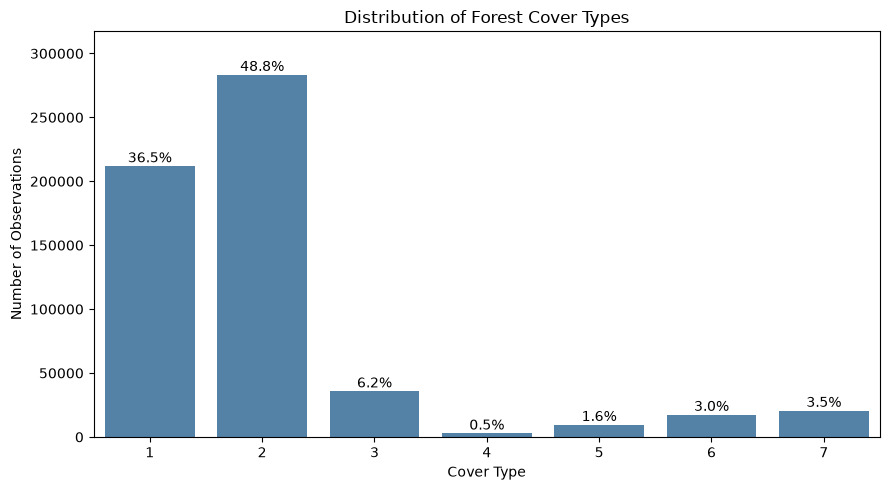
\includegraphics[
        width=0.72\linewidth
    ]{figures/data_distrib.png}
    \caption{Distribution of observations across the seven forest cover types.}
    \label{fig:class_distribution}
\end{figure}

This imbalance highlights the limitations of using accuracy alone
to evaluate classifier performance. Consequently, macro-averaged
F1-score and class-wise recall will also be considered, giving
greater visibility to performance on minority classes.


\subsection{Feature Distributions and Relationships}

The distributions of the numerical features were examined to identify
potentially discriminative variables and relationships between features.

Elevation appears particularly informative, as illustrated in
Figure~\ref{fig:elevation}. Cover types 1 and 7 are predominantly
associated with higher elevations, whereas types 3, 4 and 6
are generally found at lower elevations. However, substantial
overlap remains between certain classes, especially types 1 and 2,
and types 3 and 6.

\begin{figure}[htbp]
    \centering
    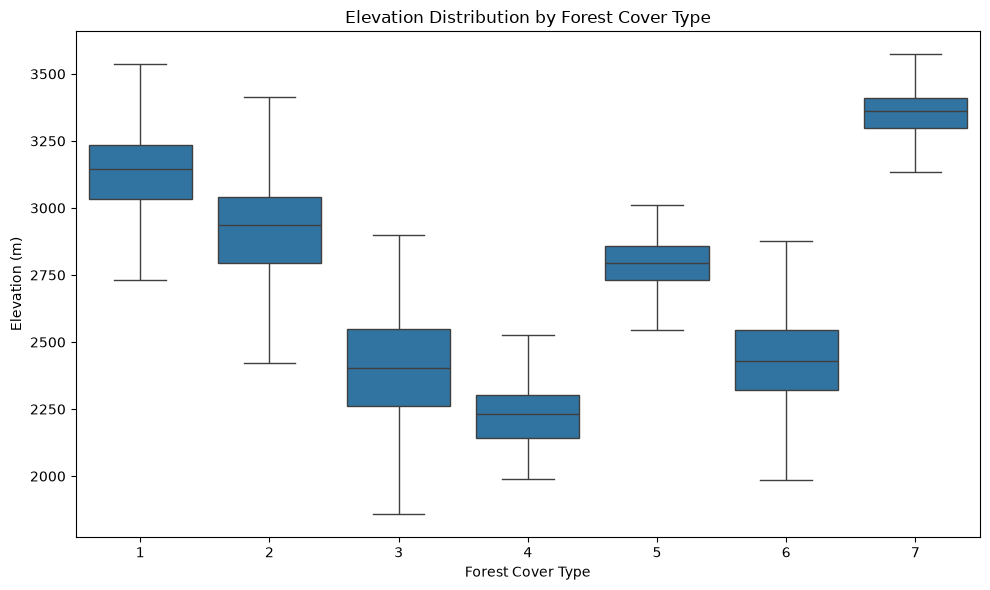
\includegraphics[
        width=0.73\linewidth
    ]{figures/altitude_boxplot.png}
    \caption{Elevation distributions for each forest cover type.
    Outliers are omitted for readability.}
    \label{fig:elevation}
\end{figure}

Other numerical variables, particularly slope and distances to
roadways and fire ignition points, also exhibit class-dependent
distributions. These observations suggest that combining multiple
features is necessary to distinguish classes with overlapping
individual distributions.

A correlation analysis further revealed some redundancy among
the numerical features. In particular, Hillshade\_9am and
Hillshade\_3pm exhibit a strong negative correlation ($r=-0.78$),
while horizontal and vertical distances to hydrology are
positively correlated ($r=0.61$).

Figure~\ref{fig:correlation_matrix} presents the correlation
matrix of the ten quantitative features. The observed correlations
indicate that some variables contain partially redundant information,
which motivates investigating dimensionality reduction through PCA.

\begin{figure}[H]
    \centering
    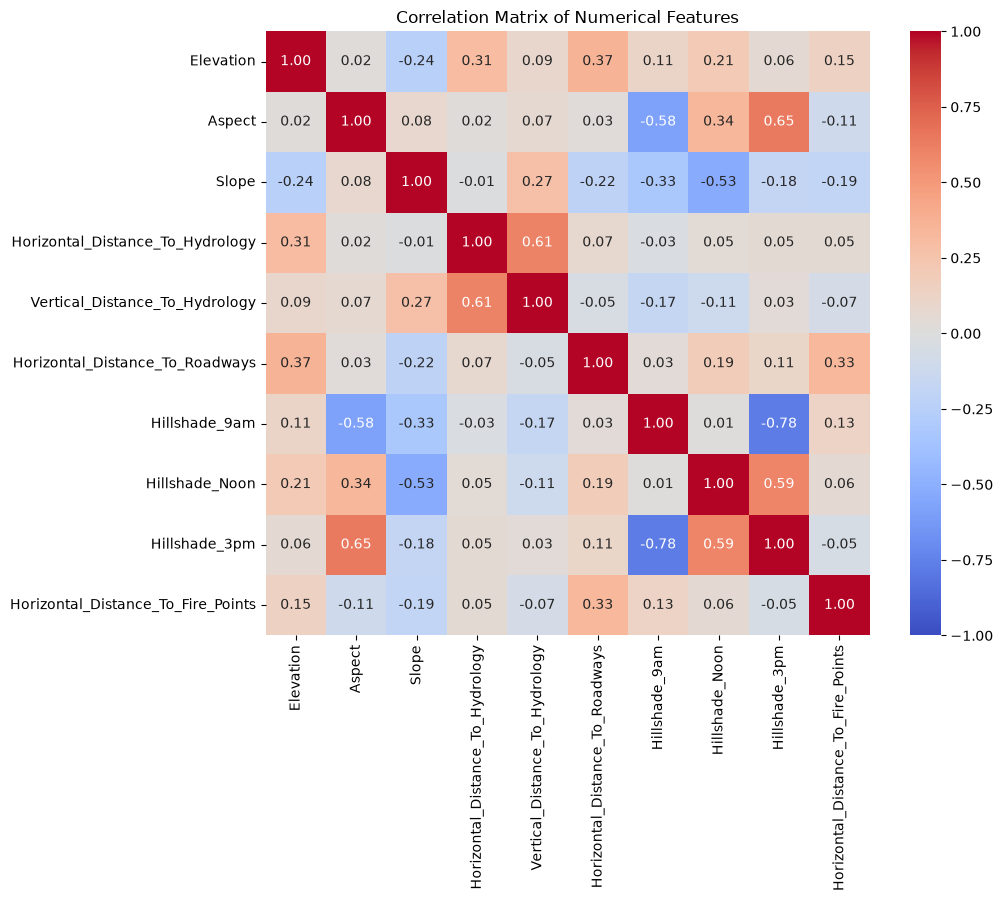
\includegraphics[
        width=0.73\linewidth
    ]{figures/corellation_heatmap.png}
    \caption{Correlation matrix of the ten quantitative
    features in the Covertype dataset.}
    \label{fig:correlation_matrix}
\end{figure}


\subsection{Implications for Classification}

Overall, the exploratory analysis highlights three important
characteristics of the dataset: substantial class imbalance,
heterogeneous feature distributions, and correlations between
certain numerical variables.

These observations motivate the use of complementary evaluation
metrics, the investigation of preprocessing techniques, and
the comparison of different feature representations.
In particular, the effect of PCA on classification performance
will be assessed experimentally rather than inferred solely
from the correlations between features.


% =========================================================
% PREPROCESSING
% =========================================================

\section{Data Preparation and Dimensionality Reduction}

\subsection{Feature Preprocessing}

Several preprocessing strategies were implemented to investigate
their influence on classification performance. Data-dependent
transformations are fitted exclusively on the training set to
avoid data leakage, while the same transformations are applied
to validation and test data.

\textbf{Feature scaling.}
The numerical features exhibit substantially different scales.
For algorithms sensitive to distances or feature magnitudes,
standardization is considered:

\begin{equation}
\widetilde{x}_{ij} =
\frac{x_{ij}-\mu_j}{\sigma_j},
\end{equation}

where $\mu_j$ and $\sigma_j$ are computed from the training set.
Scaling is automatically applied before PCA, but remains optional
when no dimensionality reduction is performed. In particular,
tree-based models are generally insensitive to monotonic feature
rescaling.

\textbf{Rare soil types.}
The exploratory analysis revealed that several soil types are
extremely uncommon, with six categories individually representing
less than 0.1\% of the observations. An optional preprocessing
step was therefore implemented to remove soil-type indicators
below a configurable frequency threshold.

However, rarity does not necessarily imply irrelevance:
some uncommon soil types are strongly associated with specific
forest cover classes. Removing them could therefore discard
useful information, particularly for minority classes.


\subsection{Cyclic Encoding of Aspect}

A particularly important preprocessing consideration concerns
the \texttt{Aspect} feature, which represents terrain orientation
as an angle between $0^\circ$ and $360^\circ$.

Although stored as a numerical variable, terrain orientation
is inherently circular. For instance, orientations of
$1^\circ$ and $359^\circ$ are physically separated by only
$2^\circ$, despite having a numerical difference of $358^\circ$.
Treating this feature as a linear variable therefore introduces
an artificial discontinuity.

This issue is particularly visible for cover type 6, whose
orientation distribution exhibits two apparent peaks near
$0^\circ$ and $360^\circ$. As illustrated in
Figure~\ref{fig:aspect_circular}, the circular representation
reveals that these peaks actually correspond to a single
continuous concentration of orientations around North.

\begin{figure}[H]
    \centering
    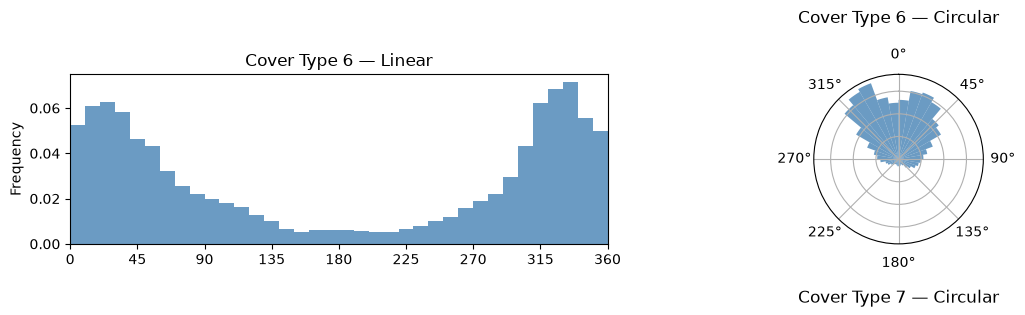
\includegraphics[
        width=0.75\linewidth,
        height=4.5cm,
        keepaspectratio
    ]{figures/aspect_circular.png}
    \caption{Linear and circular representations of terrain
    orientation for cover type 6.}
    \label{fig:aspect_circular}
\end{figure}

To account for this periodicity, an alternative representation
replaces the original angle $\theta$ with its sine and cosine:

\begin{equation}
\mathrm{Aspect}_{\cos} =
\cos\left(\frac{\pi\theta}{180}\right),
\qquad
\mathrm{Aspect}_{\sin} =
\sin\left(\frac{\pi\theta}{180}\right).
\end{equation}

This transformation maps orientations onto the unit circle,
preserving angular proximity and eliminating the artificial
discontinuity at $0^\circ/360^\circ$.


\subsection{Principal Component Analysis}

Principal Component Analysis (PCA) was investigated to reduce
feature dimensionality and potential redundancy. It projects
standardized data onto orthogonal directions of decreasing
variance.

For the covariance matrix $\Sigma$ of the standardized data,
the cumulative explained variance retained by the first $k$
principal components is

\begin{equation}
R_k =
\frac{\sum_{j=1}^{k}\lambda_j}
{\sum_{j=1}^{d}\lambda_j},
\end{equation}

where $\lambda_j$ are the eigenvalues of $\Sigma$, ordered
from largest to smallest.

Two PCA strategies were investigated:

\begin{itemize}
    \item \textbf{Numerical PCA:} PCA is applied to the
    10 standardized quantitative features, while the
    44 binary indicators are preserved.

    \item \textbf{Global PCA:} PCA is applied to all
    54 standardized features, including wilderness-area
    and soil-type indicators.
\end{itemize}

Figure~\ref{fig:pca_variance} compares the cumulative
explained variance for both approaches.

\begin{figure}[H]
    \centering

    \begin{minipage}[t]{0.48\linewidth}
        \centering
        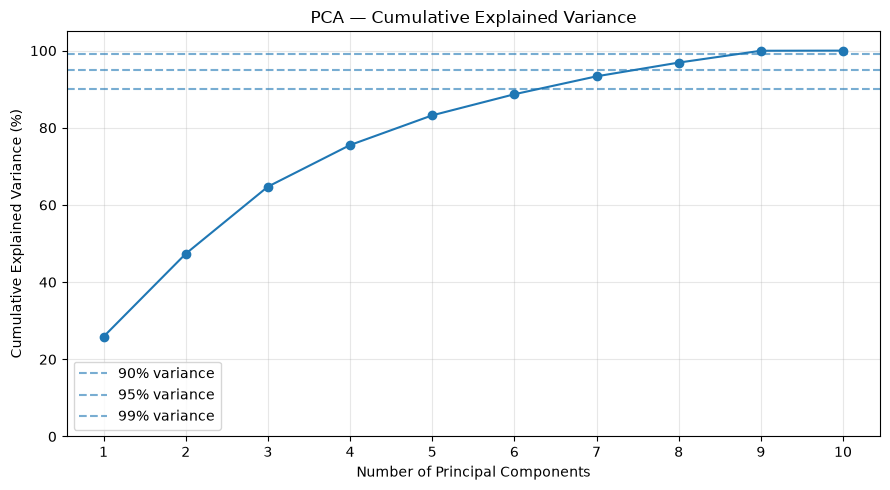
\includegraphics[
            width=\linewidth,
            height=2.9cm,
            keepaspectratio
        ]{figures/pca_numeric.png}

        {\small (a) Numerical PCA}
    \end{minipage}
    \hfill
    \begin{minipage}[t]{0.48\linewidth}
        \centering
        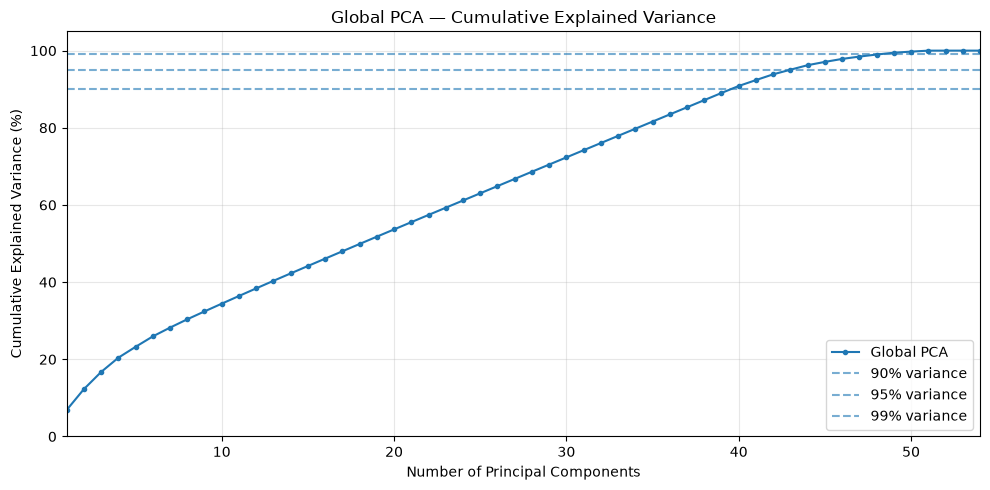
\includegraphics[
            width=\linewidth,
            height=2.9cm,
            keepaspectratio
        ]{figures/pca_global.png}

        {\small (b) Global PCA}
    \end{minipage}

    \caption{Cumulative explained variance for PCA applied
    to numerical features only (a) and to all features (b).}
    \label{fig:pca_variance}
\end{figure}

For numerical PCA, the first three principal components explain
approximately 65\% of the variance. Retaining 7, 8 and 9
components preserves respectively 90\%, 95\% and 99\% of
the variance. At the 95\% threshold, the total dimensionality
only decreases from 54 to 52 features, suggesting limited
potential computational benefits.

Global PCA requires approximately 40, 44 and 49 components
to preserve the same respective variance thresholds.
It therefore achieves greater dimensionality reduction,
but also transforms the binary indicators and reduces
their direct interpretability.

Furthermore, standardizing rare binary variables gives
them greater weight in the PCA, potentially influencing
the resulting principal components.

Importantly, PCA maximizes explained variance rather than
class separability. Consequently, neither approach can be
considered preferable based on these observations alone.
Their usefulness must be assessed experimentally through
classification performance.


% =========================================================
% CLASSIFICATION METHODS
% =========================================================

\section{Classification Methods}

Three classification algorithms were investigated: Random Forest
(RF), K-Nearest Neighbors (KNN), and Multi-Layer Perceptron (MLP).
These methods were selected to explore different approaches to
the classification problem, with particular attention to the
influence of preprocessing and hyperparameter tuning.


\subsection{Random Forest}

Random Forests were investigated for their ability to capture
nonlinear relationships and interactions between heterogeneous
features, without requiring feature scaling.

Beyond the standard hyperparameters (number of trees, maximum
depth, minimum leaf size and feature subsampling), particular
attention was given to class weighting to address the strong
imbalance identified during the exploratory analysis.

The class weights were parameterized as

\begin{equation}
w_c = \left(\frac{N}{K N_c}\right)^\alpha,
\end{equation}

where $N_c$ denotes the number of training samples belonging
to class $c$, $K=7$ is the number of classes, and $\alpha$
controls the strength of the reweighting.
This formulation allows a continuous adjustment between
uniform weighting ($\alpha=0$) and inverse-frequency
weighting ($\alpha=1$).


\subsection{K-Nearest Neighbors}

KNN was considered as a distance-based classification method,
making it particularly relevant for evaluating the influence
of feature scaling and dimensionality reduction.

The experiments focused on the number of neighbors $k$,
the distance metric (Euclidean or Manhattan), and the
weighting of neighbors. The effect of the different
preprocessing configurations was also investigated.


\subsection{Multi-Layer Perceptron}

An MLP was investigated to model nonlinear relationships
between the input features and the seven target classes.

The main parameters considered were the hidden layer
architecture, regularization strength, and learning
parameters. Particular attention was given to feature
scaling, which directly affects neural network optimization.


\subsection{Hyperparameter Optimization}

For each classifier, different hyperparameter configurations
were evaluated to improve predictive performance.
The main parameters investigated are summarized in
Table~\ref{tab:hyperparameters}.

\begin{table}[H]
\centering
\small
\begin{tabularx}{\linewidth}{@{}lX@{}}
\toprule
Model & Main hyperparameters investigated\\
\midrule
Random Forest &
Number of trees, maximum depth, minimum leaf size,
feature subsampling, class weights\\

KNN &
Number of neighbors, distance metric,
neighbor weighting\\

MLP &
Hidden layer architecture, regularization,
learning parameters\\
\bottomrule
\end{tabularx}
\caption{Main hyperparameters investigated for each classifier.}
\label{tab:hyperparameters}
\end{table}

Hyperparameters were selected primarily using validation
macro-F1, with accuracy as a complementary metric.
The experimental protocol and results are detailed in
the following sections.


% =========================================================
% EXPERIMENTAL PROTOCOL
% =========================================================

\section{Experimental Protocol}
\label{sec:experimental_protocol}

\subsection{Data Splitting}

The dataset was divided into three disjoint subsets using
stratified random sampling: 70\% for training, 15\% for
validation, and 15\% for testing. A fixed random seed
($42$) was used to ensure reproducibility.

The training set was used to fit the classifiers, while
the validation set was used for hyperparameter optimization
and model selection. The test set was reserved for the
final evaluation of the selected configurations.
All preprocessing transformations requiring parameter
estimation, including standardization and PCA, were fitted
exclusively on the training data to avoid data leakage.

Once the optimal configurations had been selected,
each classifier was retrained on the combined training
and validation sets (85\% of the dataset) before final
evaluation on the test set.


\subsection{Evaluation Metrics}

Given the substantial class imbalance observed in the
dataset, overall accuracy alone is insufficient to
evaluate classification performance. We therefore
use the macro-averaged F1-score as the primary
model selection criterion.

For each class $c$, precision and recall are defined as

\begin{equation}
P_c = \frac{TP_c}{TP_c+FP_c},
\qquad
R_c = \frac{TP_c}{TP_c+FN_c},
\end{equation}

where $TP_c$, $FP_c$, and $FN_c$ denote respectively
the true positives, false positives, and false
negatives for class $c$, considering all other
classes as negative.

The F1-score of class $c$ is the harmonic mean
of its precision and recall:

\begin{equation}
F1_c = \frac{2P_cR_c}{P_c+R_c}.
\end{equation}

The macro-averaged F1-score is then obtained
by averaging the class-specific F1-scores:

\begin{equation}
\mathrm{MacroF1} =
\frac{1}{7}\sum_{c=1}^{7}F1_c.
\end{equation}

Unlike accuracy, macro-F1 gives equal importance
to all seven classes, regardless of their frequency.
It therefore provides a more balanced assessment
of performance on minority and majority classes.

Accuracy and weighted F1-score are also reported
as complementary metrics, together with class-wise
precision, recall, and confusion matrices.
Training and prediction times are measured to
assess computational cost.


\subsection{Experimental Procedure}

For each classifier, an initial configuration was
evaluated before investigating the influence of
hyperparameters and preprocessing strategies.
The experiments included feature scaling, PCA,
and model-specific parameter optimization.

Random Forest hyperparameters were explored through
a targeted grid search, while KNN and MLP configurations
were investigated through dedicated experiments.
All configurations were compared using the same
validation set, with macro-F1 as the main selection
criterion.

Additional experiments examined model complexity,
feature importance, and the influence of training
set size where relevant.

The final configurations were selected based on
validation performance and subsequently evaluated
on the common test set. Computational times were
recorded using Python's \texttt{perf\_counter}.


% =========================================================
% RESULTS AND COMPARISONS
% =========================================================

\section{Results and Comparisons}

\subsection{Comparison of Classification Methods}

After hyperparameter optimization, the three selected classifiers
were retrained on the combined training and validation sets
(493,860 observations) and evaluated on the common test set
(87,152 observations).

Table~\ref{tab:final_results} summarizes the final predictive
performance of each model.

\begin{table}[H]
\centering
\small
\begin{tabular}{@{}lccc@{}}
\toprule
Model & Accuracy & Macro-F1 & Weighted-F1\\
\midrule
Random Forest & \textbf{0.96964} & \textbf{0.94851} & \textbf{0.96962}\\
KNN           & 0.96607 & 0.93844 & 0.96605\\
MLP           & 0.93970 & 0.90645 & 0.93959\\
\bottomrule
\end{tabular}
\caption{Final predictive performance on the test set.}
\label{tab:final_results}
\end{table}

Random Forest achieves the best overall predictive performance,
with 96.96\% accuracy and a macro-F1 of 0.9485.
KNN obtains competitive results, with a macro-F1 of 0.9384,
while MLP performs noticeably worse (0.9065).

The training and test inference times are respectively 52.68 s
and 0.51 s for RF, 0.07 s and 480.98 s for KNN, and 706.76 s
and 0.22 s for MLP.

However, overall metrics do not fully describe performance
across the seven classes. Figure~\ref{fig:class_performance}
compares class-specific F1-scores and recall values.

\begin{figure}[htbp]
    \centering
    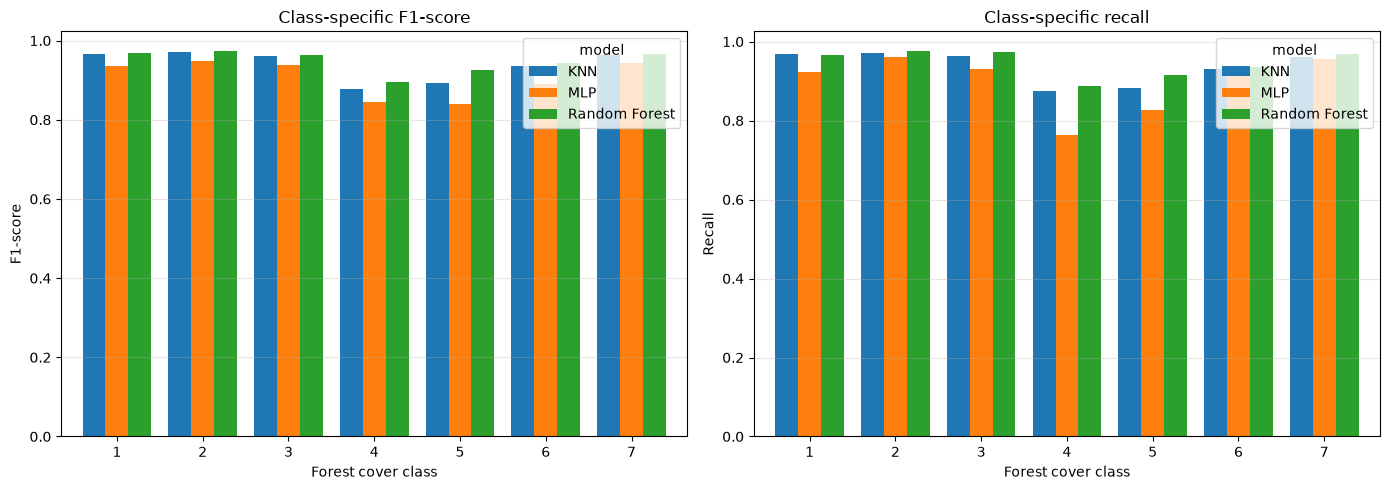
\includegraphics[
        width=0.95\linewidth,
        height=5.5cm,
        keepaspectratio
    ]{figures/class_performance.png}
    \caption{Class-specific F1-scores and recall for the
    three classifiers on the test set.}
    \label{fig:class_performance}
\end{figure}

Random Forest achieves the highest F1-score for all seven
classes, confirming that its superiority is not limited
to the majority classes. The largest differences appear
for some less represented classes, particularly class 5,
where Random Forest reaches an F1-score of 0.9254,
compared with 0.8924 for KNN and 0.8409 for MLP.


\subsection{Error Complementarity Between Classifiers}

Beyond their individual predictive performance, we investigated
whether the three classifiers make errors on the same observations.
For each pair of models, the overlap between their error sets
was measured using the Jaccard similarity:

\begin{equation}
J(A,B) =
\frac{|E_A \cap E_B|}{|E_A \cup E_B|},
\end{equation}

where $E_A$ and $E_B$ denote the sets of misclassified
test observations for models $A$ and $B$.

\begin{figure}[H]
    \centering
    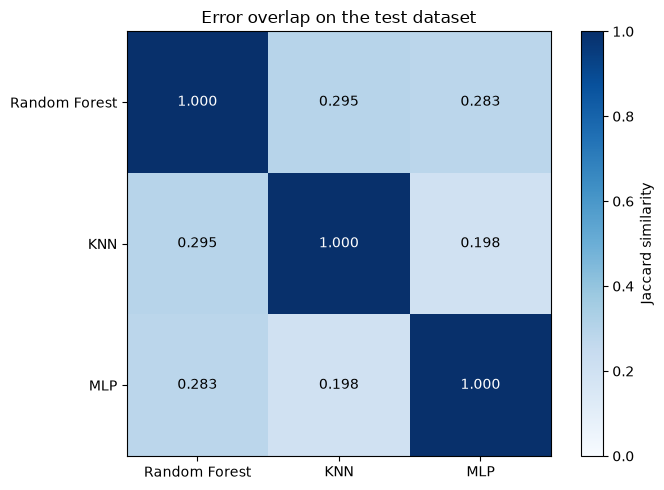
\includegraphics[
        width=0.58\linewidth
    ]{figures/error_overlap_matrix.png}
    \caption{Similarity between the classification
    errors of Random Forest, KNN, and MLP on the test set.}
    \label{fig:error_overlap_matrix}
\end{figure}

The matrix highlights the extent to which the classifiers
make similar or complementary errors.

Among the 87,152 test observations, only 905 are incorrectly
classified by all three models. At least one classifier
therefore predicts the correct class for 98.96\% of the
observations.

This suggests that the models capture partially complementary
information. Combining their predictions could be an
interesting direction for further improvement, although
the performance of such an ensemble remains to be evaluated.
The 98.96\% figure is an oracle upper bound, not the performance
of a tested ensemble.


\subsection{Random Forest Optimization}

Given its strong results, Random Forest was selected as
the final classifier. Its hyperparameters were optimized
through a targeted search over the number of trees,
feature subsampling, and class-weighting strength.

Figure~\ref{fig:rf_hyperparameters} illustrates the
influence of these parameters on validation macro-F1
and computational cost.

\begin{figure}[H]
    \centering
    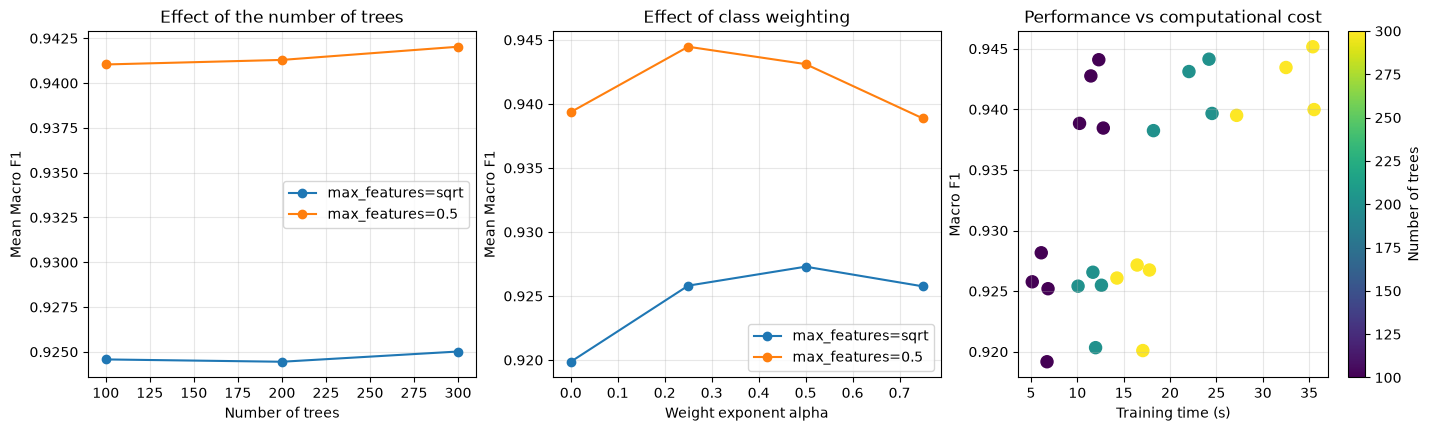
\includegraphics[
        width=0.98\linewidth,
        height=4.5cm,
        keepaspectratio
    ]{figures/rf_hyperparameters.png}
    \caption{Influence of the number of trees, class weighting,
    and training cost on Random Forest validation performance.}
    \label{fig:rf_hyperparameters}
\end{figure}

The best configuration uses 300 trees, a feature subsampling
ratio of 0.5, unlimited tree depth, a minimum leaf size
of one sample, and a class-weighting exponent $\alpha=0.25$.

It achieves a validation macro-F1 of 0.94517 and an
accuracy of 0.96715.

The experiments show that moderate class weighting
improves macro-F1, whereas stronger weighting does
not necessarily lead to better results. Increasing
the number of trees also improves performance, but
with diminishing returns and increasing computational cost.

The influence of PCA was also investigated on the
optimized Random Forest. Without PCA, the model
achieves a validation macro-F1 of 0.94517.
Numerical PCA reduces this score to 0.89751,
while global PCA yields 0.91332.

Both transformations therefore degrade predictive
performance and increase training time.
The original feature representation was consequently
retained for the final model.


\subsection{Analysis of the Selected Random Forest}

To investigate the remaining classification errors,
Figure~\ref{fig:rf_confusion_matrix} presents the
count and row-normalized confusion matrices of the optimized
Random Forest on the validation set.

\begin{figure}[H]
    \centering
    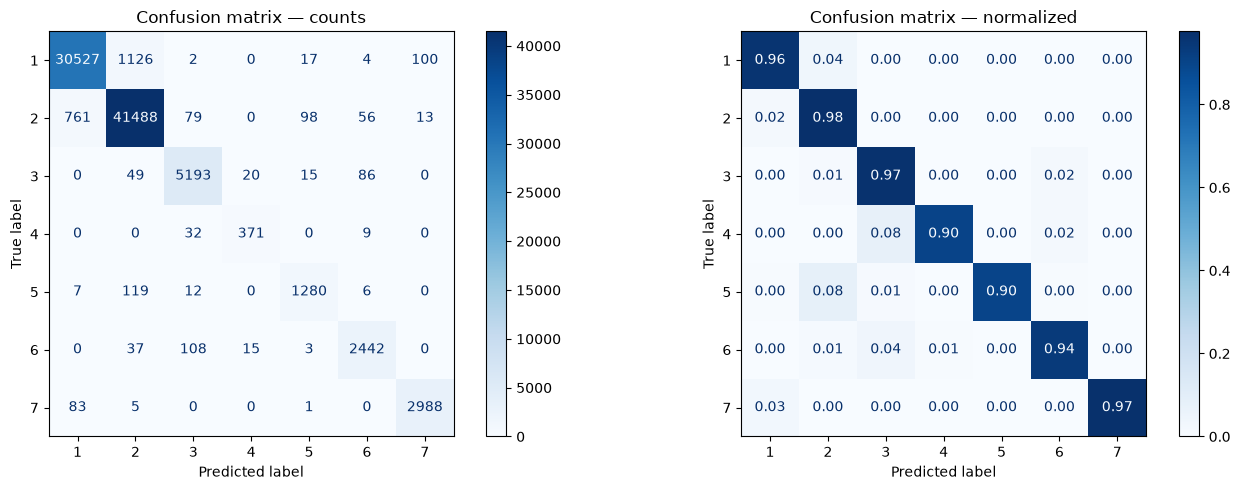
\includegraphics[
        width=0.85\linewidth,
        height=4.5cm,
        keepaspectratio
    ]{figures/rf_confusion_matrix.png}
    \caption{Count and row-normalized confusion matrices of the selected
    Random Forest on the validation set.}
    \label{fig:rf_confusion_matrix}
\end{figure}

The classifier achieves strong performance across all
seven classes. Nevertheless, classes 4 and 5 remain
the most challenging, with validation F1-scores
of 0.9071 and 0.9020, respectively.

The confusion matrix also reveals that some errors
occur between classes with overlapping environmental
characteristics, notably classes 1 and 2.

Despite these remaining errors, the relatively high
F1-scores of the minority classes indicate that
the model does not rely exclusively on the dominant
classes to achieve its overall performance.


% =========================================================
% DISCUSSION
% =========================================================

\section{Discussion and Limitations}

The experiments showed that Random Forest was the most effective
approach for this dataset, both in terms of overall performance
and classification of minority classes. One interesting result
was that PCA actually reduced performance, despite the
correlations observed between several features. This suggests
that preserving the original feature representation is
particularly useful for tree-based models. Similarly, the
experiments on class weighting showed that moderate weighting
was more effective than fully balancing the classes.

Although the results are encouraging, there are some limitations.
The hyperparameter search covered only a limited number of
configurations, and model evaluation relied on a single
stratified split. Testing different random seeds would help
determine how stable the results are. Moreover, since the
dataset contains geographical observations, a random split
does not necessarily reflect performance on entirely new
geographical areas.

Finally, the comparison of classification errors revealed
that the three models do not always make the same mistakes.
Only 905 test observations were incorrectly classified by
all three classifiers, suggesting that they capture somewhat
different information. Exploring a combination of their
predictions could therefore be an interesting next step,
although its effectiveness would need to be tested.


% =========================================================
% CONCLUSION
% =========================================================

\section{Conclusion}

The objective of this project was to develop the best possible
classifier for the Covertype dataset by exploring different
machine learning methods and preprocessing strategies.
Among Random Forest, KNN and MLP, Random Forest achieved
the best results, reaching 96.96\% accuracy and a macro-F1
score of 0.9485 on the test set. It also performed well
across all seven forest cover types, despite the significant
class imbalance.

Beyond the final scores, this project highlighted the
importance of understanding the data and testing different
model configurations. Feature engineering, hyperparameter
tuning and class weighting all played a role in our
experiments, while more complex preprocessing techniques
such as PCA did not necessarily lead to better results.
Although Random Forest proved to be the strongest model
among those tested, the analysis of classification errors
suggests that further improvements could still be explored.


% =========================================================
% REFERENCES
% =========================================================

\begin{thebibliography}{9}
\small

\bibitem{uci}
UCI Machine Learning Repository,
\emph{Covertype Dataset}.
\url{https://archive.ics.uci.edu/dataset/31/covertype}.



\end{thebibliography}


% =========================================================
% USER GUIDE
% =========================================================

\clearpage
\section*{User Guide: Running and Modifying the Experiments}

\subsection*{Installation and Setup}

The project requires Python 3.12 or later. From the repository
root, install the package and its dependencies using:

\begin{lstlisting}[language=bash]
python -m pip install -e .
\end{lstlisting}

This installs the required libraries, including NumPy, pandas,
scikit-learn, Matplotlib, Seaborn, and Jupyter's Python kernel.
The two notebooks can then be opened and executed in VS Code
or Jupyter using the corresponding Python environment.

Or with \textit{uv} :
\begin{lstlisting}[language=bash]
uv sync
\end{lstlisting}

\subsection*{Data Loading and Utilities}

The \texttt{Utils/Utils.py} module provides the shared functions
for data loading, splitting, and preprocessing.

The dataset is loaded using:

\begin{lstlisting}[language=Python]
from Utils.Utils import load_covertype_data
X, y = load_covertype_data(flatten_target=True)
\end{lstlisting}

If local Parquet files are available in \texttt{DATA/raw/},
they are loaded directly. Otherwise, the dataset is
automatically downloaded from the UCI repository and cached
locally for subsequent runs.

The \texttt{split\_data()} function creates training, validation,
and test sets. By default, it uses stratified sampling with
proportions 70\%/15\%/15\% and random seed 42.

\subsection*{Running the Notebooks}

The project is organized around two notebooks:

\begin{itemize}
    \item \texttt{DATA/data\_explore.ipynb}: dataset exploration,
    class distributions, feature analysis, preprocessing
    transformations, and PCA visualizations.

    \item \texttt{experiments.ipynb}: training, hyperparameter
    optimization, and evaluation of Random Forest, KNN,
    and MLP classifiers, followed by their final comparison.
\end{itemize}

Run the notebooks from top to bottom, starting with data
exploration if desired. The experiments notebook can also
be executed independently, as it loads and splits the data
using the shared utilities. Results and figures are displayed
directly in the notebooks.
Some experiments, particularly MLP training and hyperparameter
searches, can be time-consuming. We therefore recommend using
the saved notebook outputs to inspect the results rather than
rerunning every experiment. Individual cells can be executed
when testing specific configurations.

\subsection*{Changing Parameters}

Preprocessing options are configured through
\texttt{PreprocessingConfig} in \texttt{Utils/Utils.py}.
For example:

\begin{lstlisting}[language=Python]
from Utils.Utils import (
    PreprocessingConfig, build_preprocessor
)

config = PreprocessingConfig(
    scaling=True,
    cyclic_aspect=True,
    pca="numeric",
    pca_components=0.95
)
preprocessor = build_preprocessor(config)
\end{lstlisting}

The PCA mode can be set to \texttt{"none"},
\texttt{"numeric"}, or \texttt{"all"}.
The \texttt{pca\_components} parameter accepts either
a number of components or a retained variance ratio.
Rare soil filtering can also be enabled using
\texttt{rare\_soil\_threshold}.

Model hyperparameters can be modified directly in
\texttt{experiments.ipynb}, particularly in the
\emph{Hyperparameter Optimization} sections of each
classifier. For example, the Random Forest search grid
controls the number of trees, feature subsampling,
and class-weighting exponent.

After changing a configuration, rerun the relevant cells
and their dependencies. Model configurations are compared
primarily using validation macro-F1, while the final test
evaluation is performed after model selection.

\end{document}